\section{Solution deployment}
Our solution was deployed through Docker containers to make it more portable
and easily manageable on different platforms. Thus, the microservices, the
web app, and the monitoring tools have a dedicated Dockerfile that is
used to instantiate the specific component and wrap it into a container.
The containers are not started directly but are handled by Docker Compose
(Figure \ref{fig:docker_compose}).
This tool makes it easier for the single containers to communicate with each
other via internally resolved IP addresses and to perform replicas scaling.
The wep app and monitoring tools are exposed on external ports in order
to be accessible from outside the Docker Compose. All the microservices can
instead communicate with each other via internal addresses.


\begin{figure}
    \begin{center}
        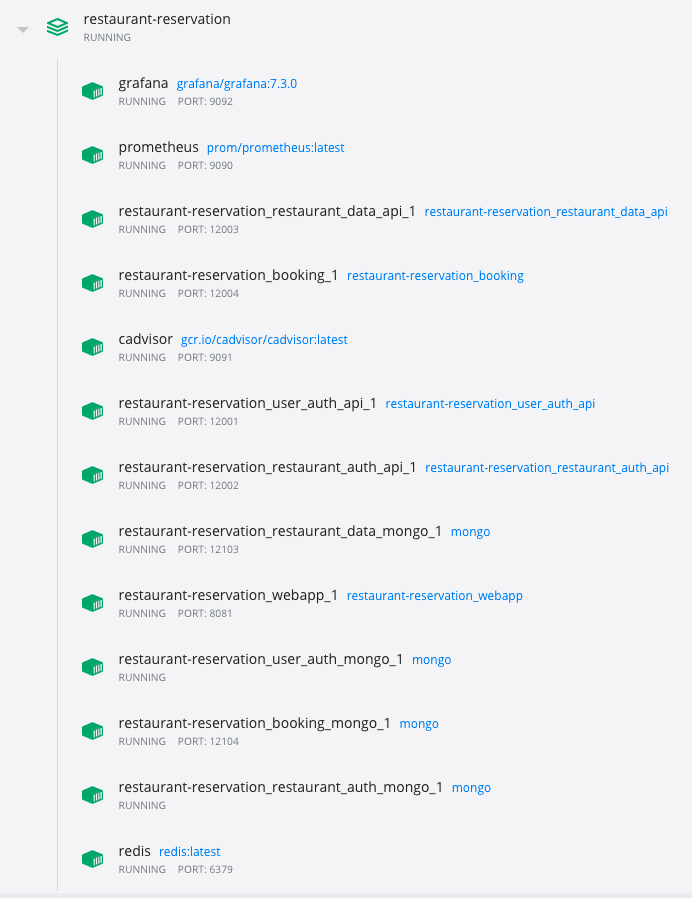
\includegraphics[height=3.5in]{./images/docker_compose.png}
    \end{center}
    \caption{Docker compose in execution.}
    \label{fig:docker_compose}
\end{figure}
